\begin{enumerate}
\item
Consider the function 
${\displaystyle{u_0(x) = \left\{\begin{array}{ll}
                      1,  & x \in [0,1/3]; \\
                      0,  & x \in (1/3,2/3); \\
                      1,  & x \in [2/3,1].
              \end{array}\right.}}$

Recall that the eigenvalues of the operator $L: C_N^2[0,1] \to C[0,1]$,
          \[ L u = -u'' \]
      are $\lambda_n = n^2 \pi^2$ for $n=0, 1, \ldots$ 
      with associated (normalized) eigenfunctions $\psi_0(x) = 1$ and 
      \[ \psi_n(x) = \sqrt{2} \cos(n\pi x), \qquad n = 1, 2, \ldots.\]
      We wish to write $u_0(x)$ as a series of the form
           \[ u_0(x) = \sum_{n=0}^\infty a_n(0) \psi_n(x),\]
      where $a_n(0) = (u_0, \psi_n)$.

%\vfill\hfill \emph{please turn over}
%\newpage 
      Compute these inner products $a_n(0) = (u_0, \psi_n)$ 
      by hand and simplify as much as possible.\\
      For $m = 0, 2, 4, 80$, plot the partial sums 
           \[ u_{0,m}(x) = \sum_{n=0}^m a_n(0) \psi_n(x).\]
      (You may superimpose these on one single, well-labeled plot if you like.)

%%%%%%%%%%%%%%%%%%%%%%%%%%%%%%%%%%%%%%%%%%%%%%%%%%%%%%%%%%%%%%%%%%%%%%%%%%%%%%%%
\item Write down a series solution to the homogeneous heat equation
\[ u_t(x,t) = u_{xx}(x,t), \qquad 0<x<1, \quad t\ge 0 \]
with Neumann boundary conditions
\[ u_x(0,t) = u_x(1,t) = 0\]
and initial condition $u(x,0) = u_0(x)$.

Create a plot showing the solution at times $t=0, 0.002, 0.05, 0.1$.\\
You will need to truncate your infinite series to show this plot.\\
Discuss how the number of terms you use in this infinite series 
affects the accuracy of your plots.

\vspace*{1em}
%%%%%%%%%%%%%%%%%%%%%%%%%%%%%%%%%%%%%%%%%%%%%%%%%%%%%%%%%%%%%%%%%%%%%%%%%%%%%%%%
\item Describe the behavior of your solution as $t\to \infty$.\\
      (Write down a formula for the solution in this limit.)

\vspace*{1em}
%%%%%%%%%%%%%%%%%%%%%%%%%%%%%%%%%%%%%%%%%%%%%%%%%%%%%%%%%%%%%%%%%%%%%%%%%%%%%%%%
\item Does the existence of the limiting solution in part~(c) contradict the fact 
      that $\lambda_0 = 0$?  Explain. 

      How would you expect the solution to the inhomogeneous heat equation
\[ u_t(x,t) = u_{xx}+ 1, \qquad 0<x<1, \quad t\ge 0 \]
with Neumann boundary conditions
\[ u_x(0,t) = u_x(1,t) = 0\]
to behave as $t\to\infty$?
\end{enumerate}

%%%%%%%%%%%%%%%%%%%%%%%%%%%%%%%%%%%%%%%%%%%%%%%%%%%%%%%%%%%%%%%%%%%%%%%%%%%%%%%%
\ifthenelse{\boolean{showsols}}{\begin{solution}
\begin{enumerate}
\item To expand $u_0(x)$ in the form
          \[ u_0(x) = \sum_{n=0}^\infty a_n(0) \psi_n(x),\]
      we must compute the coefficients $a_n(0)$.  
      For $n=0$ we compute 
        \[ a_0(0) = \int_0^1 u_0(x)\cdot 1\, \dop x 
                  = \int_0^{1/3} 1\,\dop x + \int_{2/3}^1 1\,\dop x = 2/3.\]
      For $n>0$ we have
      \begin{eqnarray*}
            a_n(0) &=& \sqrt{2} \int_0^1 u_0(x)\cos(n\pi x)\, dx  \\[0.5em]
                   &=& \sqrt{2}\Big(\int_0^{1/3} \cos(n\pi x)\, dx
                  +          \int_{2/3}^1 \cos(n\pi x)\, dx\Big) \\[0.5em]
                   &=& \sqrt{2}\Big(\Big[{\sin(n\pi x)\over n\pi}\Big]_0^{1/3}
                                   +\Big[{\sin(n\pi x)\over n\pi}\Big]_{2/3}^1 \\[0.5em]
                   &=& {\sqrt{2}(\sin(n\pi/3) - \sin(2n\pi/3)) \over n\pi}.
      \end{eqnarray*}
      [GRADERS: this last expression is sufficiently simplified for full credit.]

      Note that $\sin(2n\pi/3) = 2 \sin(n\pi/3)\cos(n\pi/3)$, and hence
       \[ \sin(n\pi/3) - \sin(2n\pi/3) = \sin(n\pi/3)(1-2\cos(n\pi/3)).\]
      Thus we have $a_n(0) = 0$ in two cases: if $n$ is a multiple of~3, 
      or if $\cos(n\pi/3) = 1/2$.  The former occurs when $n=3, 6, 9, 12, 15, \ldots$,
      whiles the latter occurs when 
        $n\pi/3 ({\rm mod}\ 2\pi) = \pi/3 \mbox{ or } 5\pi/3$,
      and hence $a_n(0) = 0$ when $n = 1+6p$ for integers $p\ge 0$ or 
      $n=-1+6p$ for integers $p\ge 1$.
      Together, this implies that for all odd integers $n$, $a_n(0)=0$.
      We end up with the partial sums shown in the following figure.
      (MATLAB code follows at the end of this solution.)
       
\begin{center}
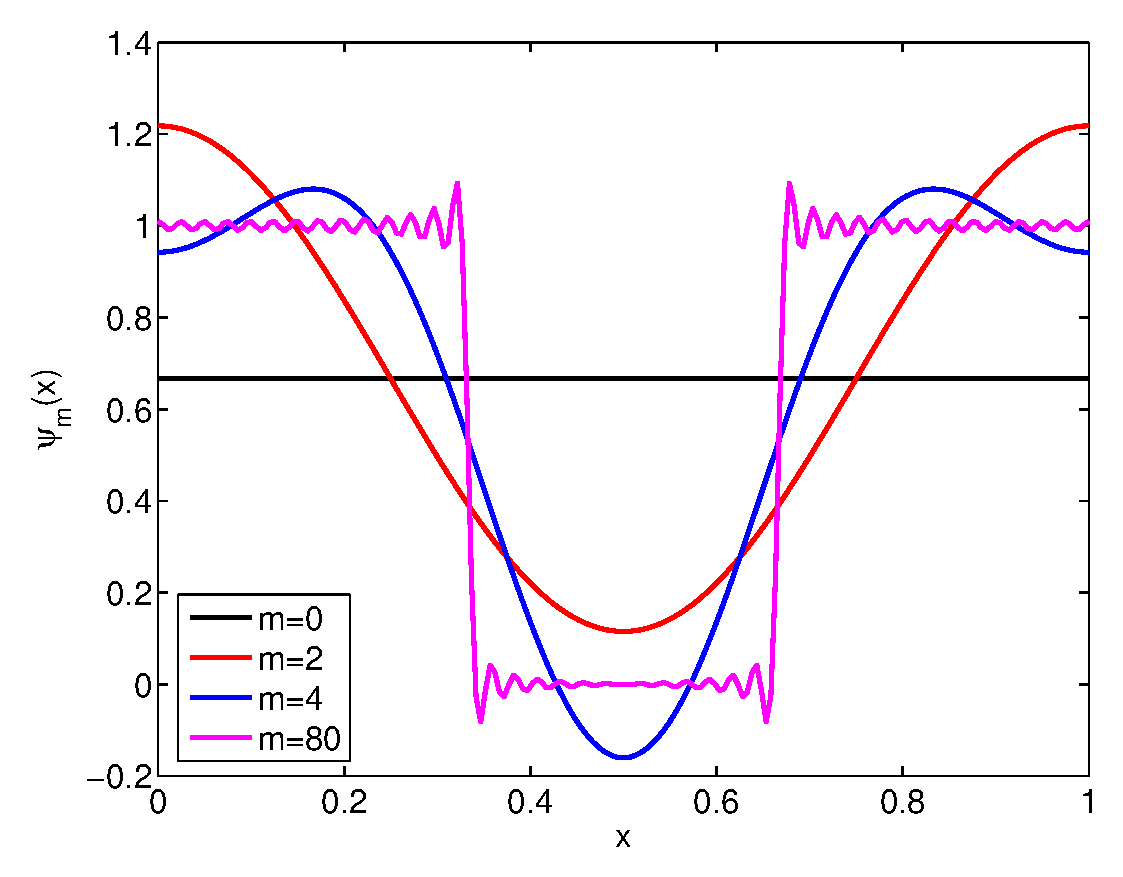
\includegraphics[scale=0.5]{heateqn1}
\end{center}

\item 
  We seek a series solution of the form
     \[ u(x,t) = \sum_{n=0}^\infty a_n(t) \psi_n(x).\]
  Using standard techniques described in class, together with the
      fact the the problem is inhomogeneous ($f(x,t) = 0$), 
      we find that
        \[ a'_n(t) + \lambda_n a_n(t) = 0.\]
      For $n=0$ we have
        \[ a'_0(t) = 0,\]
      and hence $a_0(t)$ is constant, so we conclude $a_0(t) = a_0(0) = 2/3$.
      For $n\ge 1$ we have
        \[ a_n(t) = e^{-\lambda_n t} a_n(0),\]
      where $\lambda_n = n^2\pi^2$.
      In sum, we have
        \[ u(x,t) = 2/3 + \sum_{n=1}^n e^{-\lambda_n t} 
                                a_n(0) \big(\sqrt{2} \cos(n\pi x) \big).\]

      Below we show this plot at the required times, based on taking the sum
      out to $N=20$.  While the number of terms in the series affects the accuracy
      of the solution in at early times, the importance of these extra terms 
      decreases as $t\to\infty$.
\begin{center}
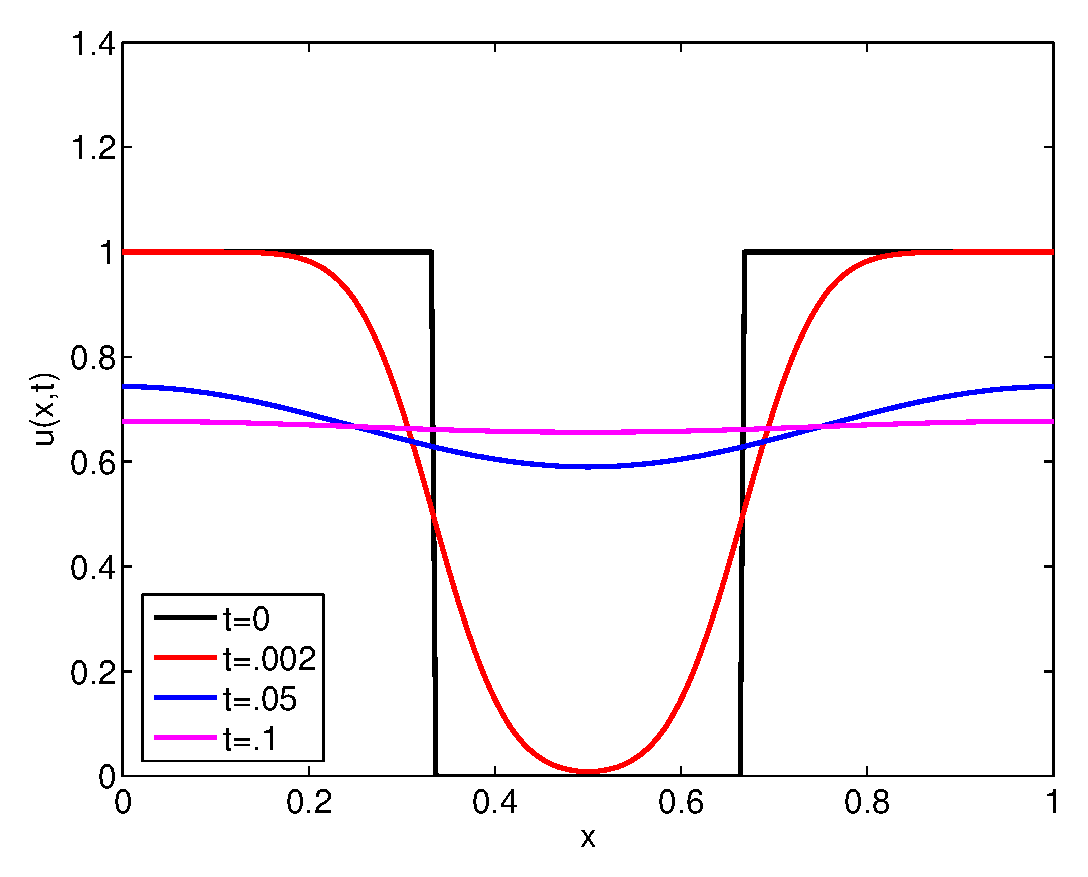
\includegraphics[scale=0.5]{heateqn2}
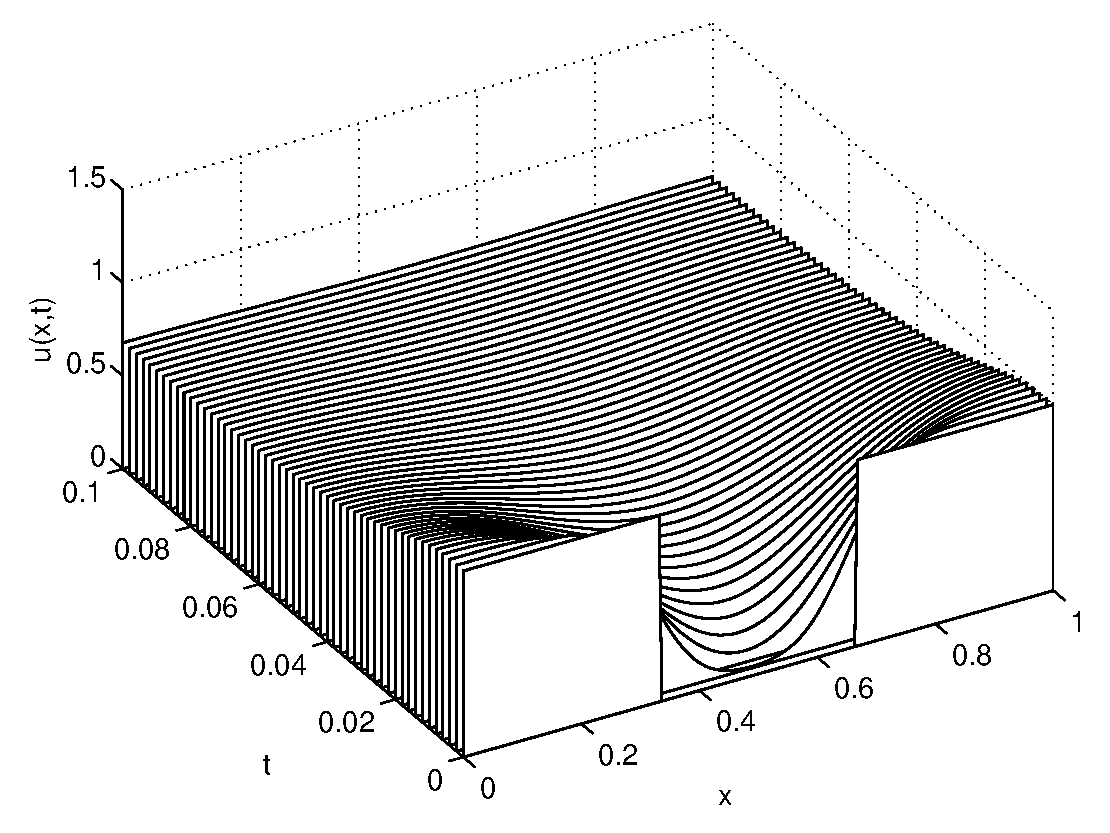
\includegraphics[scale=0.5]{heateqn3}
\end{center}

\item As is clear from the series formula in part~(b) and from the figures,
      as $t\to\infty$, $u(x,t) \to 2/3$ for all $x\in[0,1]$.

\item The existence of the limiting solution in part~(c) does not contradict
      the fact that $\lambda_0=0$.  There is no division by zero, as there is
      in the analogous steady-state problem $u_{xx} = f(x)$ with homogeneous
      Neumann conditions.  The addition of the source term adds energy to the
      system, effectively increasing the rate of change of temperature with 
      respect to time ($u_t$) by one unit.  
      This corresponds to the physical situation of pumping more
      energy into a bar that is insulated at both ends---and hence
      energy cannot escape.  Thus we expect the heat to grow as $t\to\infty$.

      The above paragraph is satisfactory for full credit, but we can actually
      be quite a bit more precise.  The eigenvalue $\lambda_0=0$ contributes
      a constant term to the solution of the PDE $u_t=u_{xx}$, and this constant 
      will be nonzero provided $(u_0,\psi_0) = \int_0^1 u_0(x)\cdot 1 \, dx \ne 0$.
      If $u_0$ has `zero mean', i.e., $\int_0^1 u_0(x)\,dx = 0$, then the solution
      to the homogeneous problem will decay as $t\to\infty$; otherwise, as $t\to\infty$
      the solution will approach the nonzero constant $(u_0,\psi_0)$.

      To write down the solution to the general inhomogeneous equation $u_t = u_{xx} + f$,
      we must expand
      \[ f(x,t) = \sum_{n=0}^\infty c_n(t) \psi_n(x).\]
      The the coefficients $a_n(t)$ in the expansion of the solution
      \[ u(x,t) = \sum_{n=0}^\infty a_n(t) \psi_n(x)\]
      obey the differential equation
      \[ a_n'(t) = -\lambda_n a_n(t) + c_n(t).\]
      As seen in class, these ODEs have the solutions
      \[ a_n(t) = e^{-\lambda_n t} a_n(0) + \int_0^t e^{-\lambda_n (t-\tau)} c_n(\tau)\,d\tau.\]
      The $a_0(t)$ case is particularly interesting: $a_0(t) = a_0(0) + \int_0^t c_0(\tau)\, d\tau$.
      Hence we cannot possibly have a steady state solution if $c_0(\tau)$ is bounded away from zero for all $\tau>0$.
 
      In the case of $f(x,t) = 1$, we have $c_0(t) = 1$ and $c_n(t) = 0$ for $n>0$, so that 
     \[ a_0(t) = a_0(0) + \int_0^t 1\, d\tau = a_0(0)+t;\]
      and for $n>0$,
     \[ a_n(t) = e^{-\lambda_n t}a_n(0),\]
      thus giving the solution
      \[ u(x,t) = a_0(0)+t + \sum_{n=1}^\infty e^{-\lambda_n t} a_n(0) \psi_n(x).\]
\end{enumerate}

\input heateqncode
\end{solution}}{}

